% use paper, or submit
% use 11 pt (preferred), 12 pt, or 10 pt only

\documentclass[letterpaper, paper,11pt]{./AAS}		% for final proceedings (20-page limit)

\usepackage{bm}
\usepackage{amsmath}
\usepackage{subfigure}
\usepackage[colorlinks=true, pdfstartview=FitV, linkcolor=black, citecolor= black, urlcolor= black]{hyperref}

\begin{document}

\subsection{$\Delta$VEGA Maneuver Implementation}
A $\Delta$VEGA orbit, also referred to as a leveraging orbit, launches from Earth with the intent to gravity assist off the body for a higher post-flyby heliocentric energy.  Leveraging orbits are classified by their nominal resonance period multiple with respect to Earth's heliocentric orbit, and we will refer to this number as "$k$." For example, a leveraging orbit that has a period roughly 3 times as large as Earth's orbit will have a $k=3$ which is represented as a 3:1 $\Delta$VEGA trajectory. The actual period of these orbits will vary either greater than or less than the nominal time due to flying by the body at a different Earth heliocentric true anomaly. Trajectories with a larger period are referred to as $k$:$1^{+} \Delta$VEGA and those with a shorter are $k$:$1^{-} \Delta$VEGA trajectories. To modify the flyby Earth true anomaly a maneuver at the aphelion (deep space maneuver) is executed.
\\\indent The deep space maneuver (DSM) and subsequent Earth launch characteristics are calculated before the tree generation in order to reduce the required number of computations within the search. We approximate the $\Delta$V requirements for both maneuvers, and their inclusion reduces the discontinuous trajectory endpoint velocities needed to patch Earth-Earth flyby sequences. Having the required aphelion $\Delta$V can also aid the optimization process initial guess. A lookup table sorted by the nominal resonance multiple ($k$) and encounter true anomalies ($\theta_{E}$) contains the resulting leveraging orbit properties and maneuver magnitudes. Due to being a rough approximation, the circular Earth orbit and coplanar trajectories assumptions are used. Finding the $\Delta$VEGA orbit parameters for a specific encounter true anomaly and $k$ begins by assuming a nominal orbit period launch and its associated $V_\infty$. The state elements are computed at Earth and the resulting aphelion radius and velocity are found. Because the intercept true anomaly is fixed, its location and the time it takes to reach the point are known. Eq.~\eqref{eq:dteqn} is the difference in time from the DSM maneuver location to the Earth gravity assist (EGA) point where $T_E$ is the orbital period of Earth.
%
\begin{equation}
	\label{eq:dteqn}
	dt = kT_E \pm T_E(\theta_E/2\pi)
\end{equation}
%
%
\begin{figure}[htb]
	\centering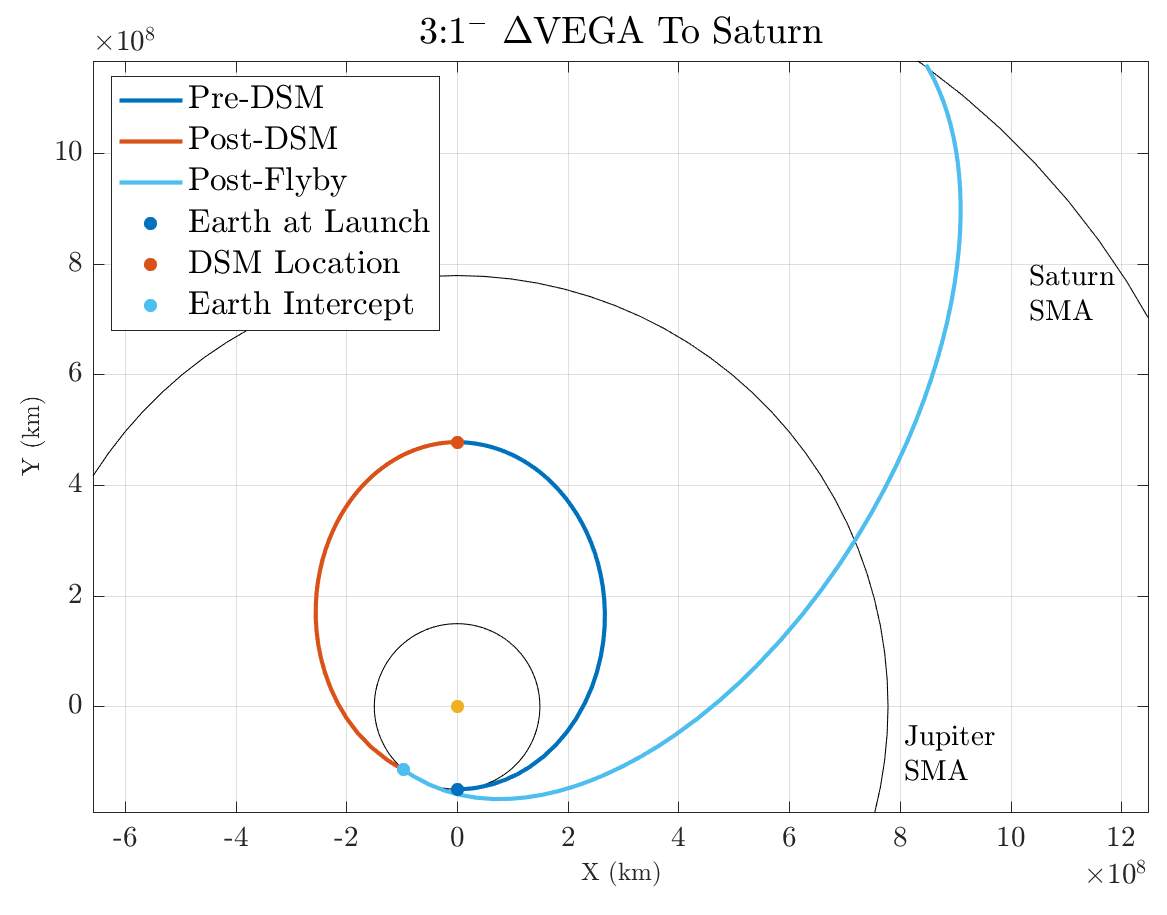
\includegraphics[width=3.5in]{./Figures/dsmmatlab}
	\caption{Example of a computed 3:$1^{-} \Delta$VEGA trajectory to Saturn's semi-major axis. The launch $V_\infty$ is 6.97 km/s and the required DSM $\Delta$V is 0.39 km/s. The EGA flyby altitude was constrained to 200 km, which yielded the highest post flyby energy.}
	\label{fig:dsmmatlab}
\end{figure}
%
\\A Lambert arc is computed between these points and the resulting initially velocity change is used to find the DSM vector. The final velocity vector is assumed to be the heliocentric velocity of the leveraging orbit at the EGA. The relative velocity, $\vec{V_\infty}$ is computed and a planar flyby of Earth can now be calculated from the tree search algorithm. Fig.~\ref{fig:dsmmatlab} illustrates an example leveraging orbit being calculated for $\theta_{E}$ = 40.$7^{\circ}$. An energy maximizing flyby and propagation to the new aphelion is added to the end of the $\Delta$VEGA orbit.
%
From testing, we noticed that as $\mid\theta_E\mid$ increased, a normal component of the DSM $\Delta$V appeared and grew larger. To limit the $\Delta$V to only a tangential component, and in return to reduce the total $\Delta$V required, a minimizer can be employed. This optimization comes at the expense of a higher launch energy and a longer flight time for trajectories with large $\mid\theta_E\mid$. Differing trends from Sims et. al. analysis of $V_\infty$ leveraging\cite{sims1994} were only noticed in high total $\Delta$V cases for each $k$ leveraging orbit family. These solutions were discarded from the lookup table due to delivering lower aphelion radii post-flyby when compared to lower total $\Delta$V leveraging orbits of the same family. The case presented in Fig.~\ref{fig:dsmmatlab} matches that discussed by Sims et. al\cite{Sims1997}.
\\\indent Now that the $\Delta$VEGA orbit properties are known, the lookup table solution can be extended to the actual solar system model in the tree search. The table values are represented in a relative frame with respect to Earth's state vector at the launch epoch. A subsequent transformation of the departure velocity and pre-EGA incoming $\vec{V_\infty}$ can be done in order to find their specific components corresponding to an Earth epoch in the Ecliptic J2000 frame. From the initial node in the tree, a set of Earth leveraging time-of-flight nodes are created corresponding to their respective $k$ and $\theta_E$ values parameters. The number of these leveraging nodes included in the initial flight time layer of the tree is directly related to the angular spacing of $\theta_E$. As the resolution becomes finer, the estimated $\Delta$V becomes more accurate. This, however, increases of the number of tree nodes created, and so for a rough idea of the trajectory search space, a coarse resolution is preferred. The discontinuous $\Delta$V post-EGA required to patch the incoming leg from the leveraging orbit and outgoing leg to the next planet node will determine if the leveraging node and its performance is effective for the transfer. Using this method, a distinction between the $\Delta$VEGA trajectory families to different outer planets can be observed.


\phantom{p. 1}
\clearpage
\bibliographystyle{./AAS_publication}
\bibliography{./referencesDSMSsection}

\end{document}
